% BDIMS Presentation Slides - LaTeX Beamer Template
% Copy this to Overleaf and compile

\documentclass[aspectratio=169]{beamer}
\usetheme{Madrid}
\usecolortheme{default}

% Packages
\usepackage{graphicx}
\usepackage{tikz}
\usepackage{listings}
\usepackage{hyperref}

% Colors
\definecolor{bloodred}{RGB}{204,0,0}
\definecolor{codegreen}{RGB}{0,128,0}
\definecolor{codegray}{RGB}{128,128,128}

% Code listing style
\lstset{
    basicstyle=\ttfamily\small,
    keywordstyle=\color{blue},
    commentstyle=\color{codegreen},
    stringstyle=\color{bloodred},
    breaklines=true,
    showstringspaces=false
}

% Title information
\title{BDIMS: Blood Donor Information Management System}
\subtitle{A Django-based Web Application}
\author{Your Team Names Here \\ Member 1 • Member 2 • Member 3 • Member 4}
\institute{Your College/University Name \\ Department of Computer Science}
\date{\today}

\begin{document}

% ============================================
% TITLE SLIDE
% ============================================
\begin{frame}
    \titlepage
\end{frame}

% ============================================
% OUTLINE
% ============================================
\begin{frame}{Outline}
    \tableofcontents
\end{frame}

% ============================================
% SECTION 1: INTRODUCTION
% ============================================
\section{Introduction}

\begin{frame}{The Problem}
    \begin{columns}
        \column{0.5\textwidth}
            \textbf{Current Challenges:}
            \begin{itemize}
                \item Slow emergency blood donor search
                \item No centralized donor database
                \item Manual eligibility tracking
                \item Poor inventory management
                \item Inefficient communication
            \end{itemize}
        
        \column{0.5\textwidth}
            \begin{center}
                \textcolor{bloodred}{\Huge \textbf{1}}\\
                \large donation saves\\
                \textcolor{bloodred}{\Huge \textbf{3}}\\
                \large lives
            \end{center}
    \end{columns}
    
    \vspace{1em}
    \textbf{Solution:} A centralized, web-based blood donation management system
\end{frame}

\begin{frame}{Project Objectives}
    \begin{enumerate}
        \item \textbf{Donor Management}
            \begin{itemize}
                \item Registration and profile management
                \item Health metrics tracking
                \item Donation history
            \end{itemize}
        
        \item \textbf{Emergency Response}
            \begin{itemize}
                \item Instant donor notification system
                \item Blood type compatibility matching
                \item Location-based donor search
            \end{itemize}
        
        \item \textbf{Administrative Tools}
            \begin{itemize}
                \item Dashboard with analytics
                \item Blood inventory management
                \item Request approval workflows
            \end{itemize}
    \end{enumerate}
\end{frame}

% ============================================
% SECTION 2: SYSTEM ARCHITECTURE
% ============================================
\section{System Architecture}

\begin{frame}{Technology Stack}
    \begin{columns}
        \column{0.5\textwidth}
            \textbf{Backend:}
            \begin{itemize}
                \item Django 5.2.8 (Python web framework)
                \item PostgreSQL (Database)
                \item Django ORM (Object-Relational Mapping)
            \end{itemize}
            
            \vspace{1em}
            \textbf{Frontend:}
            \begin{itemize}
                \item HTML5, CSS3, JavaScript
                \item Leaflet.js (Interactive maps)
                \item Chart.js (Data visualization)
            \end{itemize}
        
        \column{0.5\textwidth}
            \textbf{Tools \& APIs:}
            \begin{itemize}
                \item Git/GitHub (Version control)
                \item Nominatim (Geocoding)
                \item Browser Geolocation API
            \end{itemize}
            
            \vspace{1em}
            \textbf{Development:}
            \begin{itemize}
                \item VS Code
                \item PostgreSQL/pgAdmin
                \item Chrome DevTools
            \end{itemize}
    \end{columns}
\end{frame}

\begin{frame}{MVT Architecture}
    \begin{center}
        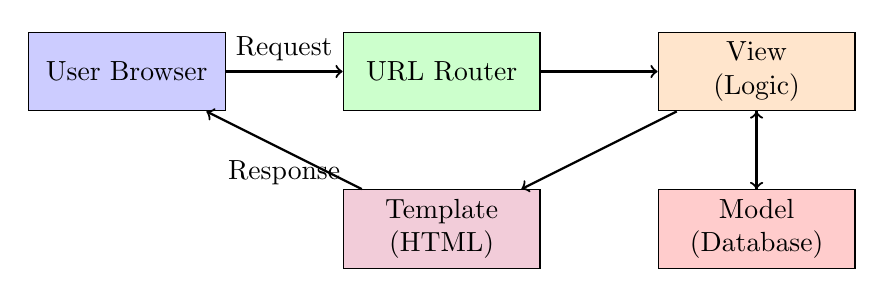
\begin{tikzpicture}[
            node distance=2cm,
            box/.style={rectangle, draw, minimum width=2.5cm, minimum height=1cm, align=center},
            arrow/.style={->, thick}
        ]
            % Nodes
            \node[box, fill=blue!20] (user) {User Browser};
            \node[box, fill=green!20, right of=user, xshift=2cm] (urls) {URL Router};
            \node[box, fill=orange!20, right of=urls, xshift=2cm] (view) {View\\(Logic)};
            \node[box, fill=red!20, below of=view] (model) {Model\\(Database)};
            \node[box, fill=purple!20, left of=model, xshift=-2cm] (template) {Template\\(HTML)};
            
            % Arrows
            \draw[arrow] (user) -- node[above] {Request} (urls);
            \draw[arrow] (urls) -- (view);
            \draw[arrow] (view) -- (model);
            \draw[arrow] (model) -- (view);
            \draw[arrow] (view) -- (template);
            \draw[arrow] (template) -- node[below] {Response} (user);
        \end{tikzpicture}
    \end{center}
    
    \vspace{0.5em}
    \textbf{Django MVT Pattern:}
    \begin{itemize}
        \item \textbf{Model:} Database tables (Donor, Request, etc.)
        \item \textbf{View:} Business logic (Python functions)
        \item \textbf{Template:} UI presentation (HTML files)
    \end{itemize}
\end{frame}

\begin{frame}{Database Schema}
    \begin{center}
        \begin{tikzpicture}[
            table/.style={rectangle split, rectangle split parts=3, draw, minimum width=3cm},
            node distance=1.5cm
        ]
            % User table
            \node[table, fill=blue!10] (user) {
                \textbf{User}
                \nodepart{two} id, username
                \nodepart{three} email, password
            };
            
            % Donor table
            \node[table, fill=green!10, right of=user, xshift=2cm] (donor) {
                \textbf{Donor}
                \nodepart{two} user\_id, blood\_group
                \nodepart{three} phone, location
            };
            
            % Request table
            \node[table, fill=orange!10, below of=donor] (request) {
                \textbf{DonationRequest}
                \nodepart{two} donor\_id, date
                \nodepart{three} status, center\_id
            };
            
            % History table
            \node[table, fill=red!10, below of=user] (history) {
                \textbf{DonationHistory}
                \nodepart{two} donor\_id, date
                \nodepart{three} units, center
            };
            
            % Emergency table
            \node[table, fill=purple!10, below of=request, yshift=-1cm] (emergency) {
                \textbf{EmergencyRequest}
                \nodepart{two} blood\_type, units
                \nodepart{three} hospital, urgency
            };
            
            % Relationships
            \draw[->, thick] (user) -- node[above] {1:1} (donor);
            \draw[->, thick] (donor) -- node[right] {1:N} (request);
            \draw[->, thick] (donor) -- node[left] {1:N} (history);
        \end{tikzpicture}
    \end{center}
\end{frame}

\begin{frame}{Project Structure}
    \begin{columns}
        \column{0.5\textwidth}
            \textbf{Modular Design:}
            \begin{itemize}
                \item \texttt{accounts/} - Authentication
                \item \texttt{donor/} - Donor features
                    \begin{itemize}
                        \item \texttt{views/} - Organized modules
                        \item \texttt{models.py} - Database
                        \item \texttt{urls.py} - Routes
                    \end{itemize}
                \item \texttt{admin\_panel/} - Admin features
                \item \texttt{utils/} - Shared helpers
            \end{itemize}
        
        \column{0.5\textwidth}
            \textbf{Views Modules:}
            \begin{itemize}
                \item \texttt{dashboard.py} - Main page
                \item \texttt{donations.py} - Scheduling
                \item \texttt{profile.py} - Account
                \item \texttt{location.py} - Maps
                \item \texttt{health.py} - Metrics
                \item \texttt{emergency.py} - Alerts
                \item \texttt{notifications.py} - Messages
            \end{itemize}
    \end{columns}
    
    \vspace{1em}
    \textit{Separation of concerns makes code maintainable and testable}
\end{frame}

% ============================================
% SECTION 3: KEY FEATURES
% ============================================
\section{Key Features}

\begin{frame}{Donor Features}
    \begin{enumerate}
        \item \textbf{Registration \& Authentication}
            \begin{itemize}
                \item Secure password hashing
                \item Role-based access (Donor/Admin)
                \item Session management
            \end{itemize}
        
        \item \textbf{Dashboard}
            \begin{itemize}
                \item Donation statistics (total, lives saved)
                \item Recent donation history
                \item Eligibility status
                \item Emergency alerts
            \end{itemize}
        
        \item \textbf{Donation Scheduling}
            \begin{itemize}
                \item 90-day eligibility check
                \item Date/time selection
                \item Center selection
                \item Admin approval workflow
            \end{itemize}
    \end{enumerate}
\end{frame}

\begin{frame}{Donor Features (Continued)}
    \begin{enumerate}
        \setcounter{enumi}{3}
        
        \item \textbf{Interactive Location Services}
            \begin{itemize}
                \item Leaflet.js map integration
                \item GPS auto-detection
                \item Reverse geocoding (coordinates → address)
                \item Find nearest hospitals
            \end{itemize}
        
        \item \textbf{Health Metrics Tracking}
            \begin{itemize}
                \item Hemoglobin level
                \item Blood pressure
                \item Weight monitoring
                \item Eligibility calculation
            \end{itemize}
        
        \item \textbf{Emergency Response}
            \begin{itemize}
                \item Blood type compatibility matching
                \item Instant notifications
                \item Quick response system
            \end{itemize}
    \end{enumerate}
\end{frame}

\begin{frame}{Admin Features}
    \begin{enumerate}
        \item \textbf{Dashboard with Analytics}
            \begin{itemize}
                \item Blood group distribution (pie chart)
                \item Donation trends (line chart)
                \item Current inventory levels
                \item Pending requests overview
            \end{itemize}
        
        \item \textbf{Donor Management}
            \begin{itemize}
                \item View all registered donors
                \item Filter by blood group, location
                \item Track donation history
                \item Donor detail pages
            \end{itemize}
        
        \item \textbf{Request Management}
            \begin{itemize}
                \item Approve/reject donation requests
                \item Track request status
                \item View donor eligibility
            \end{itemize}
    \end{enumerate}
\end{frame}

\begin{frame}{Admin Features (Continued)}
    \begin{enumerate}
        \setcounter{enumi}{3}
        
        \item \textbf{Emergency Request System}
            \begin{itemize}
                \item Create urgent blood requests
                \item Specify blood type, units, hospital
                \item Automatic donor notification
                \item Track donor responses
            \end{itemize}
        
        \item \textbf{Blood Inventory Management}
            \begin{itemize}
                \item Track available units per blood type
                \item Reserve units for requests
                \item Low stock alerts
                \item Update inventory levels
            \end{itemize}
        
        \item \textbf{Facility Management}
            \begin{itemize}
                \item Manage donation centers
                \item Hospital information
                \item Location tracking
            \end{itemize}
    \end{enumerate}
\end{frame}

% ============================================
% SECTION 4: TECHNICAL IMPLEMENTATION
% ============================================
\section{Technical Implementation}

\begin{frame}[fragile]{Django ORM Example}
    \textbf{Instead of writing SQL, we use Python objects:}
    
    \begin{lstlisting}[language=Python]
# Find all O+ donors who are eligible
eligible_donors = Donor.objects.filter(
    blood_group='O+',
    eligible=True
).order_by('last_donation_date')

# Create a new donation request
request = DonationRequest.objects.create(
    donor=donor,
    requested_date=date.today(),
    status='pending',
    donation_center=center
)

# Calculate total donations
total = DonationHistory.objects.filter(
    donor=donor
).count()
    \end{lstlisting}
    
    \textit{Django converts this to optimized SQL automatically}
\end{frame}

\begin{frame}[fragile]{Blood Compatibility Logic}
    \textbf{Matching donors to emergency requests:}
    
    \begin{lstlisting}[language=Python]
# Blood compatibility dictionary
BLOOD_COMPATIBILITY = {
    'O-': ['O-', 'O+', 'A-', 'A+', 'B-', 'B+', 'AB-', 'AB+'],
    'O+': ['O+', 'A+', 'B+', 'AB+'],
    'A-': ['A-', 'A+', 'AB-', 'AB+'],
    # ... etc
}

# Find compatible donors
def find_compatible_donors(emergency):
    # For each blood type, check what they can donate to
    for blood_type, can_donate_to in BLOOD_COMPATIBILITY.items():
        if emergency.blood_group_needed in can_donate_to:
            donors = Donor.objects.filter(
                blood_group=blood_type,
                eligible=True
            )
            notify_donors(donors, emergency)
    \end{lstlisting}
\end{frame}

\begin{frame}[fragile]{Interactive Map Integration}
    \textbf{Leaflet.js + Django backend:}
    
    \begin{lstlisting}[language=JavaScript]
// Initialize map
const map = L.map('map').setView([lat, lng], 13);

// Add OpenStreetMap tiles
L.tileLayer('https://{s}.tile.openstreetmap.org/{z}/{x}/{y}.png')
    .addTo(map);

// Handle map clicks
map.on('click', function(e) {
    // Place marker
    L.marker(e.latlng).addTo(map);
    
    // Update form fields
    document.getElementById('latitude').value = e.latlng.lat;
    document.getElementById('longitude').value = e.latlng.lng;
    
    // Reverse geocoding
    fetch(`nominatim.../reverse?lat=${lat}&lon=${lng}`)
        .then(data => updateAddressFields(data));
});
    \end{lstlisting}
\end{frame}

\begin{frame}{Security Implementation}
    \begin{columns}
        \column{0.5\textwidth}
            \textbf{Authentication \& Authorization:}
            \begin{itemize}
                \item Password hashing (PBKDF2-SHA256)
                \item Session management
                \item \texttt{@login\_required} decorator
                \item Role-based access control
            \end{itemize}
            
            \vspace{1em}
            \textbf{Data Protection:}
            \begin{itemize}
                \item CSRF token validation
                \item SQL injection prevention (ORM)
                \item XSS protection (auto-escaping)
                \item Input validation \& sanitization
            \end{itemize}
        
        \column{0.5\textwidth}
            \textbf{Best Practices:}
            \begin{itemize}
                \item Environment variables for secrets
                \item DEBUG = False in production
                \item HTTPS/SSL ready
                \item Secure cookie flags
                \item Database constraint enforcement
            \end{itemize}
            
            \vspace{1em}
            \textcolor{bloodred}{\textbf{Security is built-in, not bolted-on}}
    \end{columns}
\end{frame}

% ============================================
% SECTION 5: CHALLENGES & LEARNING
% ============================================
\section{Challenges \& Learning}

\begin{frame}{Development Challenges}
    \begin{enumerate}
        \item \textbf{Learning Curve}
            \begin{itemize}
                \item Django framework concepts (MVT, ORM, migrations)
                \item \textit{Solution:} Official documentation, tutorials, practice
            \end{itemize}
        
        \item \textbf{Database Design}
            \begin{itemize}
                \item Relationships, normalization, optimization
                \item \textit{Solution:} ER diagrams, peer review, iteration
            \end{itemize}
        
        \item \textbf{Map Integration}
            \begin{itemize}
                \item JavaScript-Python communication, API integration
                \item \textit{Solution:} AJAX, JSON, API documentation
            \end{itemize}
        
        \item \textbf{Code Organization}
            \begin{itemize}
                \item Managing 1,500+ lines of code
                \item \textit{Solution:} Modular structure, refactoring
            \end{itemize}
    \end{enumerate}
\end{frame}

\begin{frame}{What We Learned}
    \begin{columns}
        \column{0.5\textwidth}
            \textbf{Technical Skills:}
            \begin{itemize}
                \item Full-stack web development
                \item Database design \& SQL
                \item API integration
                \item Version control (Git)
                \item Security best practices
                \item Testing \& debugging
            \end{itemize}
        
        \column{0.5\textwidth}
            \textbf{Soft Skills:}
            \begin{itemize}
                \item Team collaboration
                \item Problem-solving
                \item Time management
                \item Code reviews
                \item Documentation
                \item Presentation skills
            \end{itemize}
    \end{columns}
    
    \vspace{1em}
    \begin{center}
        \textit{"From tutorial followers to confident developers"}
    \end{center}
\end{frame}

% ============================================
% SECTION 6: RESULTS & FUTURE WORK
% ============================================
\section{Results \& Future Work}

\begin{frame}{Testing \& Results}
    \textbf{Testing Methodology:}
    \begin{itemize}
        \item Manual testing with 50+ test donors
        \item Feature testing (CRUD operations)
        \item Security testing (SQL injection, XSS attempts)
        \item Cross-browser compatibility
        \item Database integrity validation
    \end{itemize}
    
    \vspace{1em}
    \textbf{Results:}
    \begin{itemize}
        \item [\checkmark] All core features functional
        \item [\checkmark] Security vulnerabilities prevented
        \item [\checkmark] Responsive design works across devices
        \item [\checkmark] Database handles concurrent users
        \item [\checkmark] 100\% URL routing success
    \end{itemize}
\end{frame}

\begin{frame}{Future Enhancements}
    \begin{columns}
        \column{0.5\textwidth}
            \textbf{Short-term (3-6 months):}
            \begin{enumerate}
                \item SMS notifications (Twilio)
                \item Email confirmations
                \item Unit test suite
                \item API documentation
                \item Performance optimization
            \end{enumerate}
        
        \column{0.5\textwidth}
            \textbf{Long-term (6-12 months):}
            \begin{enumerate}
                \item Mobile app (React Native)
                \item Machine learning donor matching
                \item Blood drive campaign module
                \item Hospital system integration
                \item QR code check-in system
            \end{enumerate}
    \end{columns}
    
    \vspace{1em}
    \begin{center}
        \textit{Scalable architecture supports future growth}
    \end{center}
\end{frame}

% ============================================
% SECTION 7: CONCLUSION
% ============================================
\section{Conclusion}

\begin{frame}{Project Impact}
    \begin{center}
        \Large \textbf{How BDIMS Helps Society}
    \end{center}
    
    \vspace{1em}
    \begin{itemize}
        \item \textbf{Saves Lives:} Quick donor matching during emergencies
        \item \textbf{Efficiency:} Reduces search time from hours to minutes
        \item \textbf{Accessibility:} Anyone can register as donor online
        \item \textbf{Transparency:} Donors track their impact (lives saved)
        \item \textbf{Safety:} Health tracking ensures donor well-being
        \item \textbf{Inventory Control:} Prevents blood wastage and shortages
    \end{itemize}
    
    \vspace{1em}
    \begin{center}
        \textcolor{bloodred}{\Large \textbf{Technology for Social Good}}
    \end{center}
\end{frame}

\begin{frame}{Conclusion}
    \textbf{Project Summary:}
    \begin{itemize}
        \item Developed comprehensive blood donation management system
        \item Achieved all objectives: donor management, emergency response, inventory control
        \item Used modern technologies: Django, PostgreSQL, Leaflet.js, Chart.js
        \item Implemented security best practices
        \item Organized modular codebase following Django conventions
    \end{itemize}
    
    \vspace{1em}
    \textbf{Key Takeaways:}
    \begin{itemize}
        \item Full-stack development experience
        \item Understanding of software engineering principles
        \item Team collaboration and project management skills
        \item Building systems that make a social impact
    \end{itemize}
\end{frame}

\begin{frame}{Thank You}
    \begin{center}
        \Huge \textbf{Thank You!}
        
        \vspace{2em}
        \Large Questions?
        
        \vspace{2em}
        \normalsize
        \textbf{Project Repository:} \\
        \url{https://github.com/YourUsername/BDIMS}
        
        \vspace{1em}
        \textbf{Contact:} \\
        your-email@example.com
    \end{center}
\end{frame}

% ============================================
% BACKUP SLIDES (For Q&A)
% ============================================
\appendix

\begin{frame}[fragile]{Backup: Code Example - Eligibility Check}
    \begin{lstlisting}[language=Python]
def can_donate(self):
    """
    Check if donor is eligible to donate blood
    
    Criteria:
    - 90 days since last donation
    - Hemoglobin >= 12.5 g/dL
    - Age 18-65
    - Weight >= 50kg
    """
    # Check time since last donation
    if self.last_donation_date:
        days_since = (date.today() - self.last_donation_date).days
        if days_since < 90:
            return False, f"Wait {90 - days_since} more days"
    
    # Check health metrics
    latest_health = self.health_metrics.latest('recorded_at')
    if latest_health.hemoglobin_level < 12.5:
        return False, "Hemoglobin too low"
    
    return True, "Eligible to donate!"
    \end{lstlisting}
\end{frame}

\begin{frame}{Backup: Database Statistics}
    \begin{center}
        \begin{tabular}{|l|r|}
            \hline
            \textbf{Database Tables} & \textbf{Fields} \\
            \hline
            User & 8 \\
            Donor & 15 \\
            DonationRequest & 10 \\
            DonationHistory & 8 \\
            EmergencyRequest & 12 \\
            HealthMetrics & 7 \\
            BloodInventory & 5 \\
            Hospital & 9 \\
            DonationCenter & 10 \\
            \hline
            \textbf{Total} & \textbf{84 fields} \\
            \hline
        \end{tabular}
    \end{center}
    
    \vspace{1em}
    \textbf{Relationships:} 12 ForeignKeys, 3 Many-to-Many \\
    \textbf{Indexes:} 11 custom indexes for performance
\end{frame}

\end{document}
